\section{ラベルの定義の設計と改訂}
\label{sec_label}
本章では，初期の7クラスのラベルを，形式，属性，媒体の3軸のラベルに作り変えた経緯を述べる．
表\ref{tab_label_history}に，定義の改訂の要点をまとめる．

\begin{table*}[t]
    \centering
    \caption{ラベルの定義の改訂の経緯}
    \label{tab_label_history}
    \small
    \begin{tabular}{>{\raggedright\arraybackslash}p{0.12\textwidth}>{\raggedright\arraybackslash}p{0.5\textwidth}>{\raggedright\arraybackslash}p{0.3\textwidth}}
        \toprule
        版 & 主な内容 & 改訂の根拠 \\
        \midrule
        初期 & 形式4値と画風4値を統合した7クラス．text は「画像の大部分が文章」 & -- \\
        草案 & 形式（1つ），属性（複数），媒体（複数），事前知識（複数）の4軸 & 強い手法の誤りが定義の境界に集中 \\
        第1版 & 形式の優先順位，お題文の範囲，媒体の複数選択の制限，事前知識に作品不明を追加 & VLM による草案の試行で判断の揺れを確認 \\
        第2版 & テロップや字幕はお題文ではなく文字とする．事前知識の軸を廃止 & お題文と事前知識の判定が全手法で低精度 \\
        第3版 & 属性の合成画像を削除し，お題文ありとその他の文字ありを文字ありに統合．媒体の CG を削除 & 統合と削除の事後の分析と下流の処理での必要性 \\
        第4版 & 文字ありをロゴや透かしを含む読める文字全般に拡張．テンプレートの主題の文をお題文と明記 & 実データの目視による誤りの分析 \\
        \bottomrule
    \end{tabular}
\end{table*}

\subsection{定義の見直しの方針}
初期の定義には次の4つの問題があった．
第1に，定義が見た目に基づいており，ボケの生成に必要な処理と対応していなかった．
第2に，画風の軸に，絵の種類と事前知識の要否という2つの観点が混ざっていた．
例えば，ある作品のキャラクターを描いたイラストは，絵の種類はイラストであるが，ボケを作るには作品の知識が要る．
第3に，空欄を含む文章や空欄を含むカルタの札のように，複数の形式に当てはまる画像の優先順位が暗黙であった．
第4に，「大部分が」「主となる」のような程度の表現が，判断者によって異なる解釈を生んだ．

そこで，ラベルを使う下流の処理から逆算して定義を決める方針とした．
表\ref{tab_downstream}に，ボケの生成で必要となる処理と，その処理の要否を決めるラベルの対応を示す．
この対応に基づき，互いに排他的な形式と，同時に成り立ちうる属性を分け，画風の軸は画像の由来を表す媒体に限定した．

\begin{table}[t]
    \centering
    \caption{下流の処理とそれを決めるラベル}
    \label{tab_downstream}
    \small
    \begin{tabular}{>{\raggedright\arraybackslash}p{0.5\linewidth}>{\raggedright\arraybackslash}p{0.38\linewidth}}
        \toprule
        下流の処理 & ラベル \\
        \midrule
        お題文の読み取りと回答の生成 & 形式のお題文 \\
        空欄の位置の検出と語の生成 & 形式の穴埋め，空欄あり \\
        カルタの記号とひらがなの読み取り & 形式のカルタ，カルタ記号あり \\
        画像中の文字の読み取り & 文字あり \\
        作品の知識の参照 & 媒体のアニメ，マンガ，ゲーム，絵画 \\
        画風に応じた生成や分析 & 媒体 \\
        \bottomrule
    \end{tabular}
\end{table}

\subsection{4軸の草案と VLM による試行}
この方針から，形式，属性，媒体，事前知識の4軸からなる草案を作成した．
形式は回答の形を制限する性質であり，カルタ，穴埋め，お題文，通常から1つを選ぶ．
属性は空欄あり，お題文あり，カルタ記号あり，それ以外の文字ありの複数選択とした．
媒体は写真，アニメ，ゲーム，CG，マンガ，テキストグラフィック，絵画，イラストの複数選択とした．
事前知識は，実在の著名人を含むか，特定の作品に由来するものを含むかの複数選択とした．

草案の文言をそのまま Qwen3-VL-8B のプロンプトにし，通常の評価用データ640枚に適用した．
その結果，テキストグラフィックの定義である「文字が記入された画像」が広すぎ，54\%の画像で選ばれた．
媒体を2つ以上選んだ画像は46\%あり，アニメの画面に「アニメとイラスト」が付くように，1つの領域に複数の媒体が付いた．
お題文の定義の例示が問いと指示に限られていたため，「〜の共通点」「〜でありそうな事」のような題目の句や，状況を設定する文がお題文と判定されなかった．
また，空欄とお題文の両方がある29枚では，形式の判定が穴埋めとお題文に分かれた．

\subsection{ボケと投稿者の選択による裏付け}
草案では，形式は実際の大喜利とペアで決め，投稿者の意図をくみ取って判定するとした．
この方針がデータで裏付けられるかを，ボケの本文と \texttt{type} 列で確かめた．
カルタのお題には，記号のひらがなから始まるボケが集中するはずである．
そこで，お題 $ q $ に付いたボケのうち，かなで始まるものの最初の文字の分布から，書き出しの集中度 $ c_q $ を(\ref{eq_concentration})で定義した．

\begin{equation}
    c_q = \max_{s \in {\mathbb S}} \frac{|\{ b \in {\mathbb B}_q : {\rm first}(b) = s \}|}{|{\mathbb B}_q|}
    \label{eq_concentration}
\end{equation}

\noindent
ここで $ {\mathbb B}_q $ はお題 $ q $ に付いたボケのうちかなで始まるものの集合，$ {\mathbb S} $ はひらがなの集合，${\rm first}(b)$ はボケ $ b $ の括弧や記号を除いた最初の文字をひらがなに変換したものである．
漢字で始まるボケは読みが分からないため除いた．

図\ref{fig_boke_signals}の左に，目視の形式ごとの書き出しの集中度の分布を示す．
縦軸が集中度であり，かなで始まるボケが5件以上ある325枚を対象とした．
右は，ボケの文字数の中央値の分布である．

\begin{figure}[t]
    \centering
    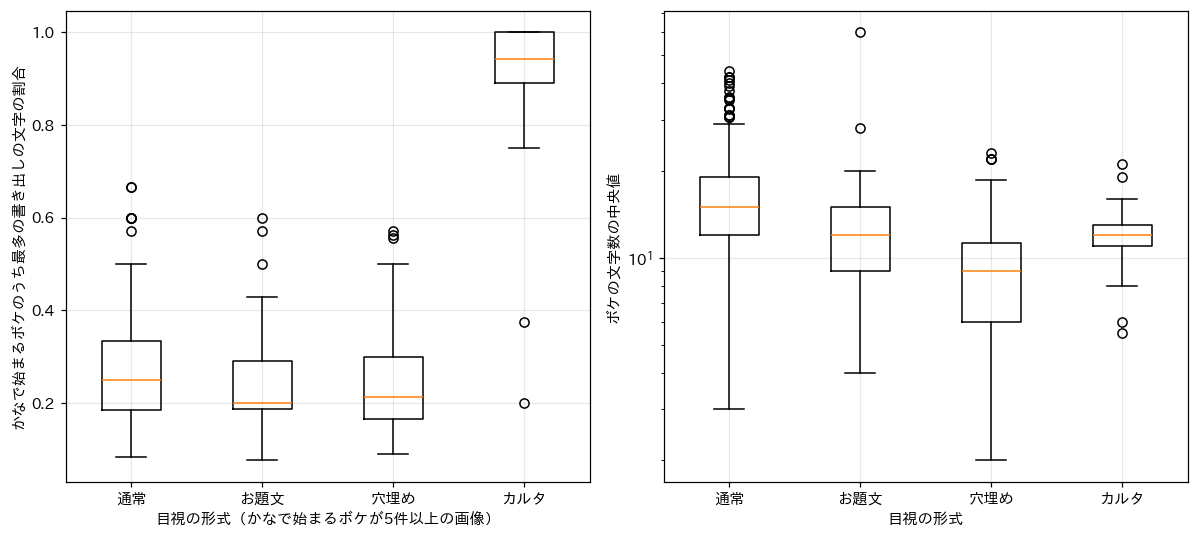
\includegraphics[width=\linewidth]{figures/fig_boke_signals.png}
    \caption{目視の形式ごとのボケの書き出しの集中度とボケの文字数の中央値}
    \label{fig_boke_signals}
\end{figure}

カルタの集中度の中央値は約0.94であり，他の形式の0.2から0.25と明確に分かれた．
集中度によるカルタの判別の AUC は 0.979 であった．
一方，ボケの文字数は形式ごとの分布の重なりが大きく，判別の手がかりとしては弱い．
\texttt{type} 列との照合では，\texttt{type} が穴埋めの52枚が全て目視でも穴埋めであり，文字の43枚のうち37枚が目視でお題文であった．
ただし，目視の穴埋めのうち \texttt{type} が穴埋めであったのは約74\%であり，投稿者の選択は適合率が高い一方で再現率は低い．
これらから，VLM の判定を主とし，ボケの書き出しと \texttt{type} 列を補助の証拠として用いる方針とした．

\subsection{第1版と第2版}
草案の試行の結果を受けて，第1版の定義を確定した．
形式は，カルタ，穴埋め，お題文，通常の順に判定し，最初に当てはまったものとする優先順位を明記した．
カルタの記号は文の一部ではなく独立した枠の中のひらがなに限り，穴埋めの空欄には黒塗りや話者に付いた空の吹き出しを含めた．
お題文には，問いと指示に加えて，題目の句，状況の設定，名前の列挙を含め，字幕や看板のように画像に元からある文字は含めないとした．
媒体は原則1つとし，複数選択は異なる媒体の領域が合成された画像に限った．
事前知識には，作品に由来するが作品名を特定できない場合を表す「作品不明」を加えた．

第1版で教師と生徒を評価したところ，事前知識の項目は教師を含む全手法で F1 が0.75未満であり，属性のお題文ありも F1 が約0.63にとどまった．
お題文ありの食い違いの多くは，テレビのテロップやアニメの字幕のように，投稿者が書き加えた文か元からある文字かを画像だけでは判別しにくいものであった．
そこで第2版では，テロップ，字幕，看板など投稿者が重畳したのではない文は，問いの形をしていてもお題文ではなく文字として扱い，テロップの中に空欄がある場合は穴埋めとした．
また，判断者の知識に依存し，教師の精度も低い事前知識の軸を廃止した．
この改訂により，教師のお題文ありの F1 は 0.63 から 0.79 に向上した．

\subsection{第3版：クラスの統合と削除}
第2版の段階で，教師と生徒の精度を下げている主な項目は，属性の合成画像，お題文ありとその他の文字ありの境界，媒体の CG であった．
クラスの統合や削除は，既存の予測と目視ラベルを同じ規則で読み替えれば，新たな学習なしに評価できる．
そこで，複数の統合と削除の案を事後に評価し，dev で選んで test で確かめた．
表\ref{tab_scheme}に，当時の最良の生徒における主な案の test のマクロ F1 を示す．

\begin{table}[t]
    \centering
    \caption{クラスの統合と削除の案の事後の評価（test のマクロ F1）}
    \label{tab_scheme}
    \small
    \begin{tabular}{llc}
        \toprule
        軸 & 案 & マクロ F1 \\
        \midrule
        \multirow{3}{*}{形式} & 現行の4クラス & 0.880 \\
         & お題文を通常に統合 & 0.923 \\
         & カルタを穴埋めに統合 & 0.884 \\
        \midrule
        \multirow{3}{*}{属性} & 現行の5項目 & 0.759 \\
         & 合成画像を削除 & 0.829 \\
         & 合成画像を削除し，文字を統合 & 0.911 \\
        \midrule
        \multirow{4}{*}{媒体} & 現行の8クラス & 0.826 \\
         & CG をイラストに統合 & 0.853 \\
         & CG と絵画をイラストに統合 & 0.877 \\
         & CG を削除 & 0.849 \\
        \bottomrule
    \end{tabular}
\end{table}

件数の少ないクラスを除けばマクロ F1 は機械的に上がるため，案の採否は精度だけでなく，表\ref{tab_downstream}の下流の処理での必要性からも判断した．
お題文を通常に統合する案は精度を最も上げたが，お題文は文字を読んで答える処理が必要な形式であり，区別が求められた種類そのものであるため採用しなかった．
合成画像は教師も生徒も F1 が0.42から0.51と最も低く，ボケの生成の処理も変えないため削除した．
お題文ありとその他の文字ありの誤りの多くは，テロップを投稿者が重畳した文とみなすかの判断にあった．
下流で必要なのは文字を読み取るかの判断のみであり，投稿者が書いた問いであるかは形式のお題文で既に表されている．
そこで2項目を文字ありに統合した．

媒体の CG は，目視で CG とした53枚のうち教師が CG と判定したのは21枚のみであり，残りは写真，ゲーム，イラスト，アニメに分散していた．
CG は，写実的な生成 AI の画像，3DCG のゲームやキャラクター，デジタルの絵にまたがっており，どのクラスに統合しても一部しか吸収できない．
そこで CG のクラス自体を削除し，3DCG や生成 AI の画像は，同じ見た目の画像を人が作った場合の媒体に振り分けることとした．
絵画をイラストに統合する案は数値では最も高かったが，絵画は F1 が0.72から0.76で判定できており，名画をもじった画像は元の作品の知識を要するため残した．
第3版で教師ラベルを付け直して生徒を学習したところ，生徒の test の3軸の平均は第2版の最良の 0.822 から 0.867〜0.897 に向上し，事後の分析による見込みの 0.880 とほぼ一致した．

\subsection{第4版：文字ありの範囲}
第3版の生徒で実データの無作為抽出160枚を確認したところ，誤りがあった41枚のうち18枚は文字ありのみの誤りであった．
そのうち17枚は，ロゴ，看板，ユニフォームの文字，画面の隅の小さな文字を，生徒が文字ありとしたものであった．
第3版の定義はロゴや透かしを除いていたが，教師はこれらを含めて回答しており，定義と教師の判定がずれていた．
文字ありの用途は，文字を手がかりにボケを分析する対象を絞ることであり，誤って含めても害は小さい．
そこで第4版では，ロゴ，透かし，著作権表示，衣服の文字なども含め，読める文字があれば文字ありとした．
文字が実際に大喜利に影響しているかは画像だけでは判断できないため，画像のラベルでは扱わず，ボケの文章を見る後段の処理で判断することとした．

さらに研究の最終段階で，ボケてのテンプレートや無地の背景に投稿者が書いた文が画像の主題である場合は，問いの形でなくてもお題文とすることを明記した．
台詞，題名，主張の文などであり，回答者はその文を読んで大喜利を作るためである．
ただし，ニュースの記事，ウェブやアプリの画面，テレビの字幕など，元からある文章を写したものは除く．

\subsection{最終の定義}
表\ref{tab_final_definition}に第4版の定義の要点を示す．
図\ref{fig_examples_final}に，最終の方法で無作為の20枚に付けたラベルを示す．
各画像の上に「形式｜属性｜媒体」の順でラベルを示し，属性の「空欄」は空欄あり，「文字」は文字あり，媒体の「テキスト」はテキストグラフィックを表す．
また，図\ref{fig_karuta_examples}にカルタの画像の例を示す．

\begin{table*}[t]
    \centering
    \caption{最終のラベルの定義（第4版）}
    \label{tab_final_definition}
    \small
    \begin{tabular}{>{\raggedright\arraybackslash}p{0.13\textwidth}>{\raggedright\arraybackslash}p{0.16\textwidth}>{\raggedright\arraybackslash}p{0.63\textwidth}}
        \toprule
        軸 & 項目 & 定義の要点 \\
        \midrule
        \multirow{4}{0.13\textwidth}{形式（1つ選択．上から順に判定）} & カルタ & ひらがな1文字が入った独立した記号がある．そのひらがなから始まる文を投稿する \\
         & 穴埋め & 語の代わりに置かれた空欄がある．○○，□，語の代わりの「？」，黒塗り，空の吹き出しを含み，顔の目隠しや文末の疑問符は含まない \\
         & お題文 & 投稿者が書き加えた，回答者に向けた問い，指示，題目の句，状況の設定，名前の列挙，テンプレートの主題の文がある．テロップ，字幕，看板など元からある文字は含まない \\
         & 通常 & 上記以外 \\
        \midrule
        \multirow{3}{0.13\textwidth}{属性（複数選択）} & 空欄あり & 穴埋めの空欄がある \\
         & カルタ記号あり & カルタの記号がある \\
         & 文字あり & ロゴ，透かし，衣服の文字を含め，読める文字がある．カルタ記号のひらがなのみの場合は除く \\
        \midrule
        \multirow{7}{0.13\textwidth}{媒体（原則1つ．合成画像では面積の約2割以上を占める各領域の媒体）} & 写真 & 現実の写真．実写の映像やフィギュアを撮影したものを含む \\
         & アニメ & アニメのスクリーンショット \\
         & ゲーム & ゲーム画面のキャプチャ \\
         & マンガ & 漫画作品から切り抜いたコマ．漫画風の一枚絵はイラスト \\
         & テキストグラフィック & 文字や記号が主体で，写真や絵がほとんどない画像 \\
         & 絵画 & 古典的な絵画．浮世絵などの版画と，写真に撮った絵画を含む \\
         & イラスト & 上記以外の絵．3DCG や生成 AI の画像は見た目に応じて振り分ける \\
        \bottomrule
    \end{tabular}
\end{table*}

\begin{figure*}[t]
    \centering
    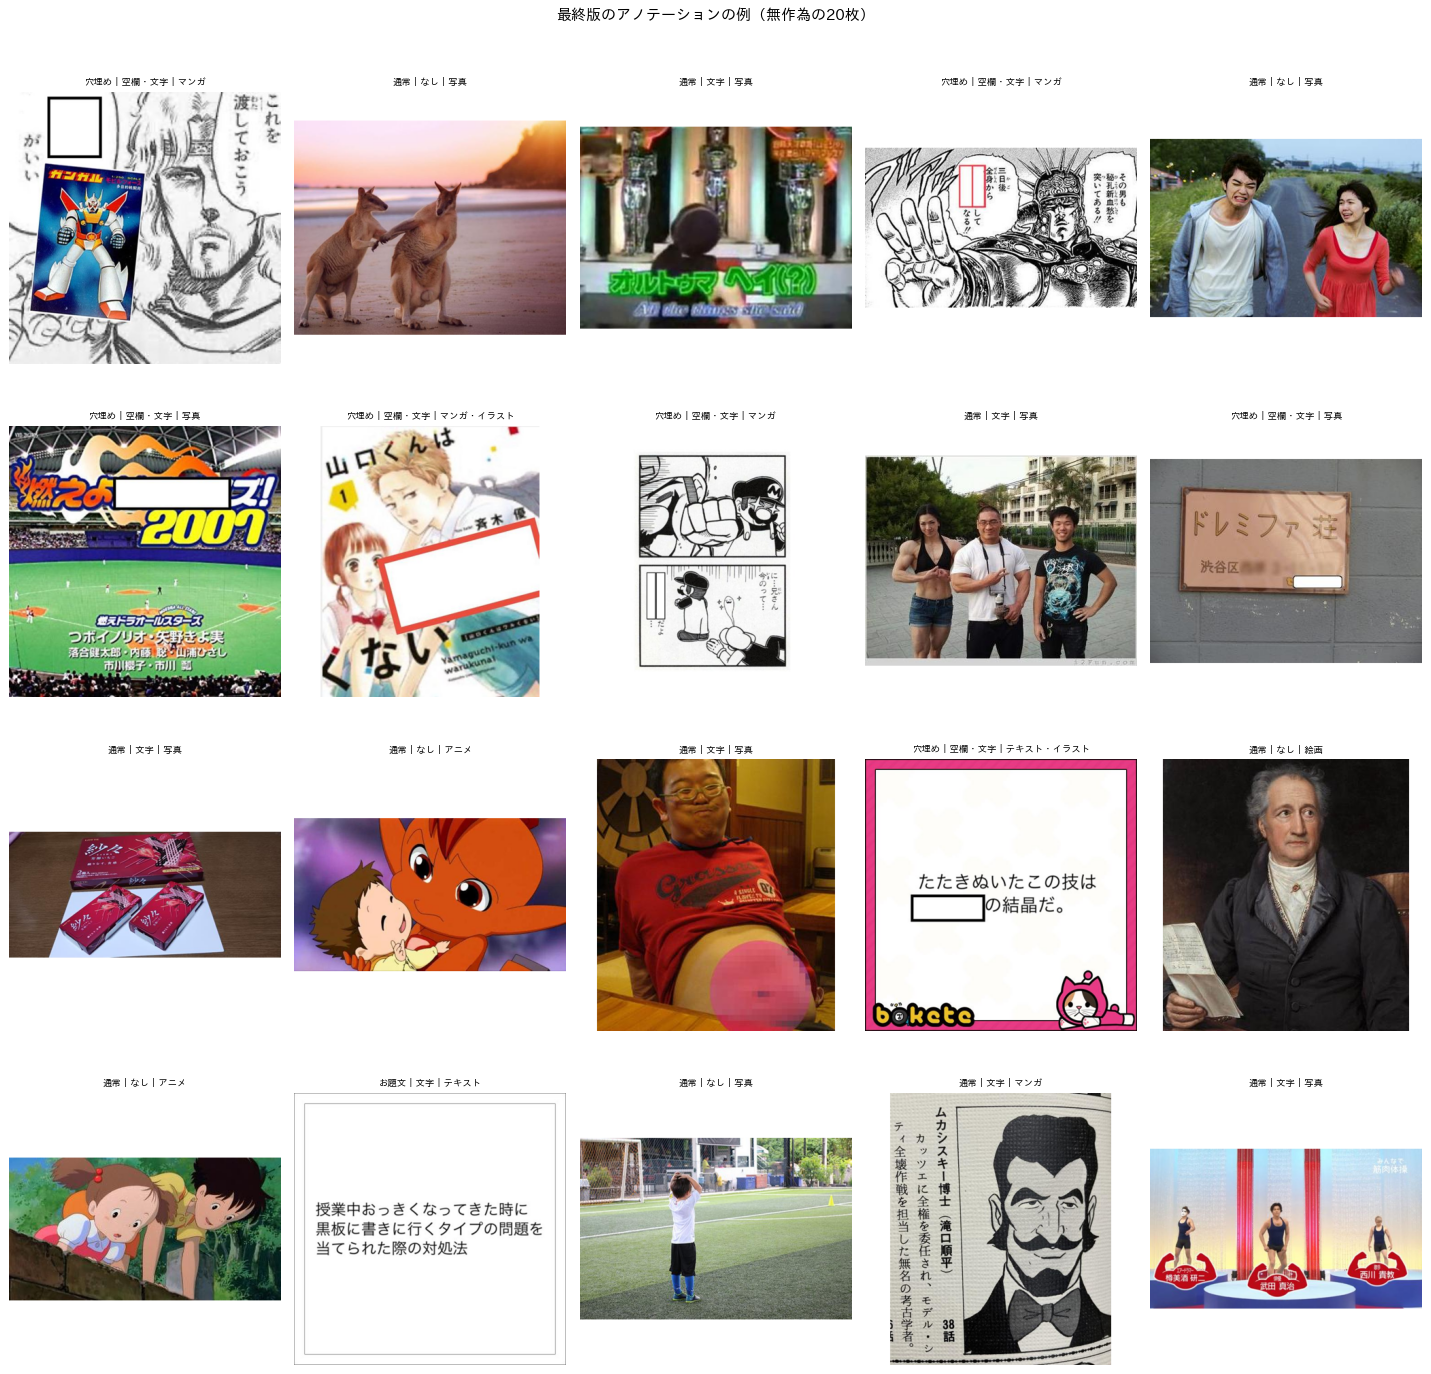
\includegraphics[width=0.85\textwidth]{figures/fig_examples_final.png}
    \caption{最終の方法によるアノテーションの例（無作為の20枚）}
    \label{fig_examples_final}
\end{figure*}

\begin{figure*}[t]
    \centering
    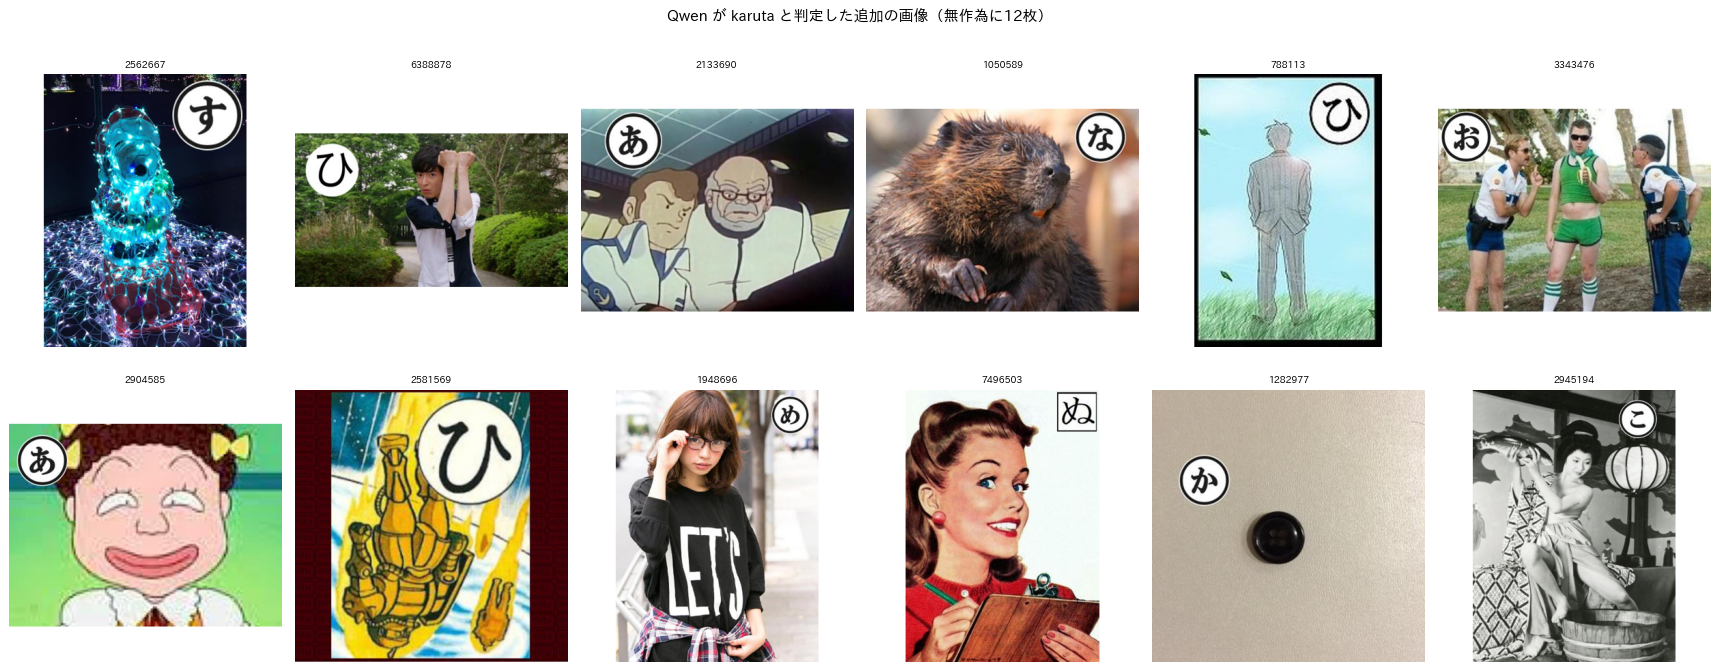
\includegraphics[width=0.9\textwidth]{figures/fig_karuta_examples.png}
    \caption{教師がカルタと判定した画像の例．画像の上の数字はお題 ID}
    \label{fig_karuta_examples}
\end{figure*}
